\chapter{Marco Metodológico}
\label{cap:metodologia}

El presente capítulo detalla la metodología utilizada para el desarrollo de la investigación, estructurada bajo el estándar CRISP-DM (\textit{Cross-Industry Standard Process for Data Mining}), la cual proporciona un enfoque iterativo y riguroso para la minería de datos, garantizando que los modelos analíticos desarrollados respondan directamente a las necesidades del negocio y del entorno clínico y administrativo (\cite{wirth2000crisp}). A continuación, se describen las fases del proyecto, comenzando por la comprensión del problema y la caracterización de los datos.

\section{Fase 1: Entendimiento del problema (\textit{Business Understanding})}
\label{sec:entendimiento_problema}

El cáncer represente a una de las principales causas de mortalidad prematura y morbilidad en Chile, generando una presión asistencial y económica crítica sobre la red pública de salud. Sin embargo, a pesar de la urgtencia epidemiológica de esta enfermedad, la caracterización de los pacientes con cáncer se ha sustentado históricamente en estudios clínicos locales, segmentados por centros hospitalarios específicos o basados en muestras reducidas, tal como se evidenció en el capítulo de estado del arte (sección \ref{sec:caracterizacion_cohortes_estadistica}). Esta fragmentación de la información dificulta contar con una visión nacional consolidada que refleje la complejidad operativa, las trayectorias intrahospitalarias y los múltiples factores asociados a la severidad de los episodios a lo largo de todo el sistema de salud.

Actualmente, el sistema de Grupos Relacionados por el Diagnóstico (GRD) reúne información estandarizada de los egresos hospitalarios de la red pública, representando una fuente masiva y valiosa de datos a nivel nacional, sin embargo, esta información no ha sido explotada en el ámbito oncológico. En la práctica, estos datos se utilizan principalmente con fines de facturación y asignación presupuestaria \cite{fonasa2023_presupuesto, ClapesUC2023}, impidiendo responder preguntas fundamentales sobre los factores de riesgo clínico (como mortalidad y severidad) y el consumo de recursos en pacientes oncológicos. En consecuencia, existe una brecha crítica en la ausencia de una caracterización que permita identificar perfiles clínico, demográfico y hospitalarios para apoyar la toma de decisiones operativas.

Frente a la necesidad de transformar estos registros administrativos en una herramienta de inteligencia sanitaria, el objetivo de este estudio consiste en caracterizar perfiles de riesgo operativo en oncología, diferenciando los factores que determinan la severidad, consumo de recursos y mortalidad de los pacientes internados en Chile. Para lograrlo, se aplicarán técnicas de aprendizaje automático y modelos de Inteligencia Artificial Explicable (XAI) sobre los datos del sistema GRD correspondientes al periodo 2019-2024, con el fin de superar el enfoque tradicional, aislando las variables más determinantes del proceso asistencial para contribuir al diseño de estrategias de gestión hospitalaria basadas en evidencia.


\section{Fase 2: Comprensión y preparación inicial de los datos}
\label{sec:preparacion_datos}

% Esta fase tiene por objetivo adquirir los datos brutos provenientes de los registros administrativos, evaluar su calidad estructural y aplicar los primeros filtros lógicos para definir las cohortes de estudio. Dado el volumen y la complejidad de los archivos anuales, el proceso se dividió en las siguientes etapas:


% La fase de preparación de datos abarcó las técnicas de minería y preprocesamiento necesarias para transformar los registros brutos en un formato tabular estructurado, apto para el entrenamiento de los algoritmos de aprendizaje automático. Este proceso se ejecutó de manera sistemática y secuencial, comenzando por el análisis de cardinalidad y culminando con el tratamiento de valores nulos y formatos inconsistentes temporales.

\subsection{Adquisición e identificación de formatos}

Los datos utilizados en esta investigación fueron extraídos del repositorio de datos abiertos del Fondo Nacional de Salud (FONASA), específicamente del visor público del sistema GRD correspondiente al período comprendido entre 2019 y 2024. Estos registros se encontraban particionados en seis archivos de texto plano (\texttt{.txt}) delimitados por barras verticales (\textit{pipes}), con un tamaño total superior a 4,4 GB (\cite{fonasa_visor_grd}). Cabe mencionar que, como medida de respaldo, se creó una carpeta en Google Drive para almacenar los archivos originales.

% citar el google Drive: https://drive.google.com/drive/u/2/folders/1zD3vm7UgkVBE50dETQlDX_b5yjS9wCFS

Debido a que la recopilación de estos datos estuvo sujeta a distintas políticas de gestión de la información, se detectaron discrepancias en los formatos de origen. Por ello, el primer desafío técnico consistió en abordar la heterogeneidad en los formatos de escritura de cada archivo. Para ello, se diseñó un algoritmo utilizando la librería \textit{chardet} para detectar y validar la codificación (\textit{encoding}) nativa de cada archivo, identificando, por ejemplo, codificaciones como \texttt{UTF-8}, \texttt{UTF-8-SIG} y \texttt{UTF-16}.

Posteriormente, se realizó un análisis de la consistencia estructural de los archivos, enfocado en la arquitectura de sus variables. Mediante operaciones de conjuntos, evaluando la diferencia asimétrica entre las listas de columnas de cada año, se mapearon sistemáticamente las características de cada archivo e identificaron sus diferencias. Adicionalmente, para cada año se analizó la existencia de filas problemáticas que presentaran una cantidad de columnas superior al resto de los registros del archivo.

Cabe destacar que este escaneo estructural tuvo como propósito identificar las variables que fueron añadidas, eliminadas o renombradas por FONASA a lo largo del período comprendido entre 2019 y 2024. Esta etapa resulta crítica dentro del ciclo de vida del dato propuesto por CRISP-DM, ya que detectar estas variaciones temporales de forma temprana permite consolidar una lectura robusta de las bases de datos para su posterior procesamiento y evitar la propagación de errores de dimensionalidad, como la generación de valores \textit{NaN} de origen estructural durante la etapa de modelamiento. De este modo, se aseguró que las características seleccionadas para los modelos de aprendizaje automático mantuvieran continuidad histórica dentro de la red pública de salud.


% https://public.tableau.com/views/PropuestaTableroGRD/PropuestaTableroGRD?%3AshowVizHome=no


\subsection{Limpieza básica y clasificación de la cohorte oncológica}

Para evitar sesgos de selección y permitir que los algoritmos de aprendizaje automático aprendieran patrones contrastantes, el diseño experimental contempló mantener a la población sin diagnóstico oncológico como grupo de control, asignándole la etiqueta \texttt{SIN\_CANCER}.

El primer paso de limpieza consistió en la exclusión de todos los episodios hospitalarios catalogados como registros inválidos, definidos como aquellas filas que carecían de un diagnóstico principal registrado (columna \texttt{DIAGNOSTICO1} nula). Posteriormente, se diseñó un algoritmo de clasificación basado en expresiones regulares para agrupar los códigos CIE-10, mediante el cual todos los diagnósticos pertenecientes al capítulo II de la clasificación CIE-10 (códigos comprendidos entre C00 y C97) fueron categorizados en 15 tipologías oncológicas, según la localización del tumor maligno.

Además, para garantizar una captura exhaustiva de la morbilidad oncológica, la clasificación se ejecutó mediante una estrategia de escaneo dual. Además de evaluar el diagnóstico principal, se verificó la existencia de un registro oncológico en el resto de los diagnósticos:
\begin{enumerate}
    \item \textbf{Detección de cáncer principal:} Inicialmente se evaluó la columna \texttt{DIAGNOSTICO1}. Los pacientes cuyo motivo principal de ingreso correspondía a un código de neoplasia maligna fueron etiquetados bajo la categoría de tipo de cáncer principal (\texttt{TIPO\_DIAGNOSTICO\_ONCO: PRINCIPAL}).
    \item \textbf{Detección de cáncer secundario:} Para los pacientes que inicialmente no presentaban cáncer en el diagnóstico principal, se implementó un escaneo iterativo sobre las 34 columnas de diagnósticos secundarios (\texttt{DIAGNOSTICO2} a \texttt{DIAGNOSTICO35}). Si el algoritmo detectaba un código oncológico en cualquiera de estas comorbilidades, el paciente era reclasificado y etiquetado bajo la categoría de tipo de cáncer secundario (\texttt{TIPO\_DIAGNOSTICO\_ONCO: SECUNDARIO}).
\end{enumerate}

Finalmente, aquellos episodios que superaron ambos escaneos sin presentar códigos comprendidos entre C00 y C97 fueron asignados definitivamente al grupo de control, es decir, sin cáncer (\texttt{CATEGORIA\_CANCER: SIN\_CANCER}, \texttt{TIPO\_DIAGNOSTICO\_ONCO: SIN\_CANCER}).

Cabe mencionar que, este procedimiento de clasificación de la cohorte oncológica y del grupo de control puede visualizarse en la Figura \ref{fig:clasificacion_cohorte}.

\begin{figure}[htbp]
    \centering
	\captionsetup{justification=centering}
    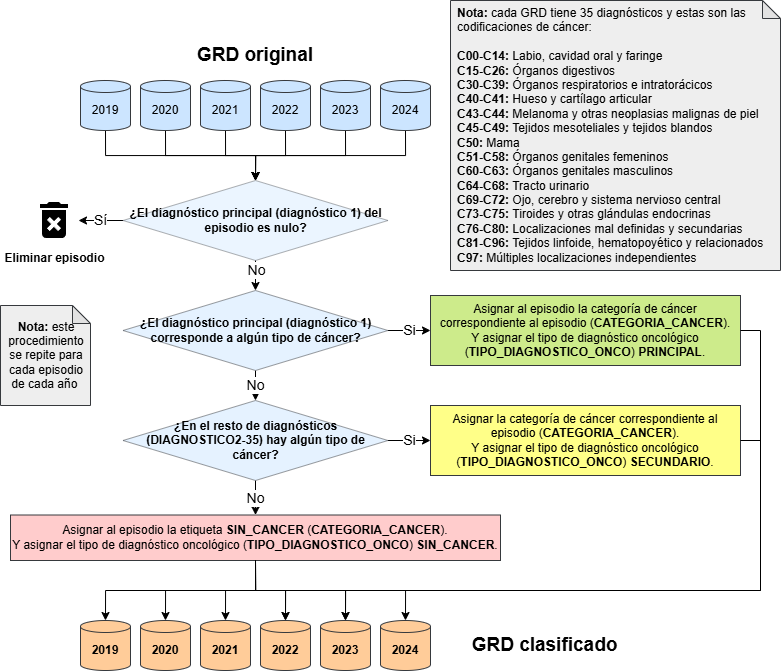
\includegraphics[width=1\textwidth]{images/clasificacion_cohorte.png}

	\caption[Procedimiento para la clasificación de la cohorte oncológica y control.]{Procedimiento para la clasificación de la cohorte oncológica y control.\\Fuente: Elaboraci\'on propia, 2026.}
    \label{fig:clasificacion_cohorte}
\end{figure}


\subsection{Análisis de variables identificadoras}

Para no comprometer la capacidad de generalización de los modelos durante la etapa de modelado, se evaluó el rol de las variables identificadoras (como el ID del paciente, los códigos de hospitales y las identificaciones médicas), ya que las variables con alta cardinalidad (es decir, con un elevado número de categorías únicas) en conjuntos de datos clínicos suelen actuar como ruido estadístico y pueden comprometer la capacidad de inferencia de los modelos.

Por ello, primero se cuantificó la frecuencia de episodios por paciente único a través de la variable \texttt{CIP\_ENCRIPTADO}. Cabe mencionar que, aunque se detecten pacientes con múltiples episodios históricos (readmisiones), se determinó que el enfoque metodológico de esta investigación requería analizar los episodios hospitalarios como instancias independientes de consumo de recursos asistenciales. De este modo, cada hospitalización se procesó como una unidad de análisis discreta.

De manera análoga, se analizó la distribución de los identificadores de los hospitales (\texttt{COD\_HOSPITAL}) y de los profesionales responsables de la intervención y del alta (\texttt{MEDICOINTERV1} y \texttt{MEDICOALTA}), con el fin de evaluar su potencial como variables predictoras a partir de su cardinalidad.

Finalmente, es importante destacar que los datos utilizados en esta investigación se encuentran completamente anonimizados y que no es posible revertir los identificadores de los pacientes (\texttt{CIP\_ENCRIPTADO}) y médicos (\texttt{MEDICOALTA}, \texttt{MEDICOINTERV1}). En consecuencia, el tratamiento de esta información se realizó exclusivamente con fines estadísticos, sin permitir la identificación de personas naturales, en concordancia con las disposiciones establecidas en la Ley N° 19.628 sobre Protección de la Vida Privada de la República de Chile (\cite{ley19628}). Bajo estas condiciones, el estudio no requirió el acceso a datos personales identificables ni la obtención de consentimiento informado.

\subsection{Análisis de variables temporales}

Después de analizar las variables identificadoras, se realizó un escaneo automatizado para evaluar la integridad y la coherencia de las distintas fechas registradas en los episodios hospitalarios de GRD (como \texttt{FECHA\_NACIMIENTO}, \texttt{FECHA\_INGRESO}, \texttt{FECHAALTA}, fechas de traslado \texttt{FECHATRASLADO1-9} y las fechas de los procedimientos quirúrgicos como \texttt{FECHAPROCEDIMIENTO1} y \texttt{FECHAINTERV1}). Esto se debe a que las variables temporales constituyen un eje crítico para medir el consumo de recursos, la severidad o la mortalidad de los episodios, ya que permiten calcular, por ejemplo, los tiempos de estancia o el riesgo asociado a la edad.

Cabe destacar que el algoritmo de saneamiento identificó y abordó tres desafíos estructurales relacionados con las variables temporales:

\begin{itemize}
    \item \textbf{Múltiples formatos de origen:} El algoritmo identificó fechas codificadas en distintos formatos (como el estándar ISO \texttt{YYYY-MM-DD}, formatos locales \texttt{DD-MM-YYYY} o cadenas concatenadas \texttt{YYYYMMDD}). Para ello, se emplearon técnicas de expresiones regulares y análisis de patrones que permitieron estandarizar todas las fechas al formato \texttt{Datetime} de Pandas, garantizando la coherencia temporal en todo el conjunto de datos.
    \item \textbf{Gestión de valores predeterminados del sistema:} Se detectaron registros en los que los campos temporales vacíos del sistema clínico original habían sido autocompletados con valores por defecto (como \texttt{"0000-00-00"} o \texttt{"00000000"}). En consecuencia, el algoritmo los reclasificó como valores nulos reales (\textit{missing values}) para evitar distorsiones en los cálculos derivados de las variables temporales.
    \item \textbf{Validación de rangos lógicos:} Finalmente, se excluyeron los registros cuyas fechas transformadas presentaban años lógicamente imposibles o correspondían a fechas futuras incompatibles con un contexto clínico coherente (por ejemplo, fechas de nacimiento con años posteriores a la fecha de extracción de los datos).
\end{itemize}


\subsection{Análisis de distribución y cardinalidad de variables categóricas}

Dada la naturaleza de los registros GRD, gran parte de sus características descriptivas correspondía a variables categóricas (como el tipo de alta, la procedencia, el sexo, la etnia y los procedimientos). Por ello, se implementó una estrategia basada en matrices de frecuencias para comparar la distribución de las categorías de cada variable entre la cohorte oncológica y el grupo control, así como su comportamiento a lo largo del período 2019--2024. Este análisis permitió evaluar el potencial predictivo de cada variable mediante el estudio de su cardinalidad y de la prevalencia de sus categorías, además de detectar posibles errores de codificación y elevados niveles de datos faltantes que pudieran requerir procesos de homologación, imputación o exclusión.

En específico, este análisis permitió determinar qué variables categóricas se conservarían, cuáles requerirían una transformación (mediante agrupación o binarización para reducir su cardinalidad) y cuáles serían descartadas. En consecuencia, esta etapa constituyó un requisito previo para construir posteriormente un conjunto de datos más estable y con una menor cantidad de variables generadas mediante One-Hot Encoding, reduciendo así el ruido y la alta dimensionalidad que podrían afectar el desempeño de los modelos de aprendizaje automático.

Cabe mencionar que, este preprocesamiento incluyó técnicas de normalización computacional (como la codificación UTF-8 y la eliminación de acentos y caracteres especiales) y la homologación semántica de categorías para fusionar respuestas equivalentes (por ejemplo, homologar \texttt{NINGUNA} y \texttt{SIN INFORMACION} bajo la categoría única \texttt{NINGUNO} en variables sociodemográficas). Además, los valores originalmente ausentes en los campos de texto (como cadenas vacías o el valor \texttt{"NaN"}) fueron imputados explícitamente bajo la categoría \texttt{"NULOS"}, preservando así la información asociada al patrón de ausencia de registros.


\subsection{Limpieza y normalización de variables numéricas}
El análisis descriptivo e imputación de las variables cuantitativas requirió un enfoque minucioso para garantizar la validez estadística de los atributos de consumo de recursos. Entre las características analizadas destacaron los pesos relativos de los Grupos Relacionados por el Diagnóstico (peso del episodio) y los tiempos operativos expresados numéricamente.

El primer desafío consistió en la inconsistencia del formato de captura. Se detectaron caracteres alfabéticos residuales y el uso indistinto de comas y puntos como separadores decimales en distintos años del repositorio GRD. Estos errores tipográficos fueron corregidos programáticamente (mediante expresiones regulares) para homogeneizar las columnas hacia representaciones de punto flotante (\textit{floats}). 

Una vez estandarizados los formatos, se calcularon métricas de resumen estadístico (media, mediana, desviación estándar, rango intercuartílico y coeficiente de variación) de forma estratificada para la cohorte oncológica, el grupo de control y la población total. Este análisis estratificado permitió detectar asimetrías severas en las distribuciones e identificar valores atípicos (\textit{outliers}) mediante el método del Rango Intercuartílico (IQR). A diferencia de enfoques puramente estadísticos donde los \textit{outliers} suelen eliminarse para estabilizar las varianzas, en el contexto del aprendizaje automático aplicado a la gestión clínica de alta complejidad, estos valores atípicos (por ejemplo, pacientes con pesos relativos excepcionalmente altos) contienen información crítica sobre episodios de severidad extrema, por lo que fueron retenidos intencionalmente en el conjunto de entrenamiento.

\subsection{Procesamiento de las variables objetivo (\textit{Targets})}
El objetivo del presente trabajo consistió en desarrollar un análisis basado en Inteligencia Artificial Explicable para perfilar tres resultados asistenciales críticos en pacientes oncológicos. Para ello, se derivaron tres variables objetivo (\textit{targets}) independientes a partir de los datos brutos, sobre las cuales se entrenarían posteriormente los algoritmos de clasificación. La discretización se realizó de la siguiente manera:

\begin{enumerate}
    \item \textbf{Mortalidad hospitalaria (Clasificación binaria):} A partir de la variable categórica de condición al egreso (\texttt{TIPOALTA}), se generó una variable dicotómica donde el valor ``1'' representó la condición de fallecido intrahospitalario, mientras que el valor ``0'' agrupó al resto de las categorías de supervivencia (alta médica, traslados, fugas).
    \item \textbf{Nivel de severidad (Clasificación multiclase ordinal):} Se procesó la variable \texttt{IR\_29301\_SEVERIDAD}, filtrando los códigos desconocidos y estandarizando la escala numérica para establecer cuatro niveles ordinales clínicos: menor (0), moderado (1), mayor (2) y extremo (3).
    \item \textbf{Consumo de recursos (Clasificación multiclase categórica):} Dado que el peso relativo calculado por el algoritmo de 3M (\texttt{IR\_29301\_PESO}) es un valor numérico continuo con una distribución fuertemente sesgada a la derecha, se optó por discretizar dicha métrica para facilitar la identificación de perfiles de riesgo operativo. La variable fue transformada en terciles estadísticamente balanceados, generando las categorías ordinales de consumo de recursos: Bajo (0), Medio (1) y Alto (2).
\end{enumerate}

Es fundamental destacar que, para evitar cualquier forma de ruido estocástico o distorsión durante la evaluación de los modelos, **se aplicó una política estricta de eliminación de registros nulos sobre las variables objetivo**. A diferencia de las variables predictoras (donde los nulos pueden ser imputados), cualquier episodio clínico que careciera de información explícita sobre su condición de egreso, severidad o peso relativo fue eliminado de forma irreversible de la cohorte de estudio, evitando la falsificación del *Ground Truth*.

\subsection{Simulación de impacto y reducción de cardinalidad}
Antes de someter las variables explicativas (\textit{features}) categóricas al modelo algorítmico, se implementó una estrategia sistemática para gestionar la alta cardinalidad y tratar los valores ausentes mediante técnicas de reducción de dimensionalidad semántica.

En lugar de aplicar codificación \textit{One-Hot} indiscriminada (lo que multiplicaría exponencialmente la complejidad del modelo provocando \textit{overfitting}), se utilizaron diccionarios de homologación basados en conocimiento experto. Por ejemplo, se agruparon 57 provincias administrativas distintas en 16 macro-categorías correspondientes a las Regiones del país, y se consolidaron decenas de registros de pueblos originarios bajo una única variable binaria representativa (\texttt{ES\_PUEBLO\_ORIGINARIO}).

Previo a la eliminación de cualquier categoría residual clasificada como "Desconocida" o de la depuración final de nulos, se diseñó e integró un simulador de impacto. Este algoritmo calculaba preventivamente cuántos episodios del grupo oncológico o del grupo de control se perderían al suprimir los datos incompletos y, fundamentalmente, verificaba si dichas eliminaciones afectaban asimétricamente a las clases de los \textit{targets} (como los episodios de pacientes fallecidos). Si la simulación indicaba que la pérdida de registros superaba los márgenes estadísticos aceptables o afectaba de manera desproporcionada a la clase minoritaria, la variable defectuosa era retenida y sus nulos encapsulados como una categoría propia (\texttt{NULOS}), asegurando así la preservación de la representatividad clínica de la base de datos maestra.

\subsection{Ingeniería de características (\textit{Feature Engineering})}
Con el fin de maximizar la capacidad predictiva de los algoritmos de aprendizaje automático sobre los episodios GRD, se diseñó e implementó un proceso de ingeniería de características. El objetivo de este paso fue construir variables derivadas sintéticas que capturaran la "intensidad" y el contexto del caso clínico con mayor fidelidad que los datos tabulares crudos. 

A partir de la iteración y el análisis lógico de las variables base, se extrajeron las siguientes características operativas y clínicas:
\begin{itemize}
    \item \textbf{Carga de enfermedad (Comorbilidades):} La literatura epidemiológica demuestra que un paciente con múltiples patologías concurrentes presenta un riesgo inherentemente mayor de complicaciones. Para cuantificar esto, se generaron tres variables: \texttt{NUM\_COMORBILIDADES} (conteo de diagnósticos secundarios válidos, excluyendo el cáncer base), \texttt{CARGA\_ONCOLOGICA} (conteo estricto de códigos neoplásicos para diferenciar tumores únicos de enfermedades metastásicas) y \texttt{COMORBILIDAD\_PRINCIPAL} (mapeo del diagnóstico secundario primario hacia uno de los 16 macrogrupos del CIE-10).
    \item \textbf{Bandera quirúrgica (\textit{Surgical Flag}):} En la gestión de camas y recursos hospitalarios, la distinción entre un manejo médico y uno quirúrgico es estructural. Mediante la inspección de la raíz del código del procedimiento principal (\texttt{PROCEDIMIENTO1}), se derivó la variable binaria \texttt{ES\_QUIRURGICO} (1 si implicaba intervención de pabellón o incisión, y 0 en caso contrario).
    \item \textbf{Variables cronológicas (Edad y Días de estadía):} Aprovechando las fechas depuradas en etapas anteriores, se calculó la \texttt{EDAD} del paciente al momento del ingreso y la variable \texttt{DIAS\_ESTADIA} (diferencia en días entre la fecha de ingreso y la fecha de alta). 
\end{itemize}

Tras la creación de estas variables derivadas, se ejecutó un filtro final y estricto sobre el conjunto de datos. Cualquier episodio que contuviera errores irreversibles en el cálculo de estas métricas (como edades negativas producto de errores de digitación de los prestadores en el año de nacimiento) fue forzado a nulo y posteriormente eliminado, garantizando un \textit{dataset} analítico libre de ruidos sistémicos o valores espurios.

\subsection{Análisis de correlación y reducción de multicolinealidad}
Para evitar que los modelos de aprendizaje automático sufrieran de sobreajuste por redundancia de información (\textit{overfitting}) o que la posterior interpretabilidad algorítmica (valores SHAP) diluyera la importancia de las características entre variables gemelas, se realizó un análisis profundo de correlación y asociación.

En primera instancia, se calculó la correlación de Spearman para todas las variables numéricas y derivadas (como Días de Estadía y Número de Procedimientos), comprobando la ausencia de dependencias lineales perfectas que justificaran su eliminación cruzada.

Posteriormente, debido a la predominancia de características cualitativas, se calculó la matriz de asociación \textit{V de Cramer} para todo el bloque de variables categóricas. Este escaneo estadístico detectó interacciones estructurales casi perfectas ($>0.99$), lo que obligó a justificar la exclusión de determinadas variables del modelo final:
\begin{itemize}
    \item Se excluyó la variable \texttt{TIPO\_ACTIVIDAD} debido a su correlación absoluta con el \textit{target} \texttt{SEVERIDAD}. Esta dependencia ocurría porque el algoritmo agrupador de 3M asigna el tipo de actividad evaluando los mismos parámetros clínicos que definen la severidad del episodio, lo que constituiría un caso crítico de fuga de datos (\textit{Data Leakage}).
    \item Se excluyó la variable \texttt{TIPO\_SERVICIO\_SALUD} por su solapamiento perfecto con la variable \texttt{REGION}. Dado que la red de salud en Chile obedece a una distribución geográfica, mantener ambas variables inducía ruido estocástico; se optó por conservar únicamente la Región territorial por su mayor valor interpretativo para la salud pública.
\end{itemize}

\subsection{Codificación One-Hot y partición estratificada del conjunto de datos}
Para convertir el conjunto de datos final en una matriz matemática compatible con los tensores de los algoritmos de \textit{Machine Learning}, se aplicó la técnica de codificación \textit{One-Hot Encoding} (OHE) sobre las variables categóricas nominales, transformando cada categoría en una característica binaria independiente. Durante este proceso, se utilizó el parámetro de reducción estructural (\textit{drop\_first=True}) para eliminar la categoría base de cada variable, mitigando la multicolinealidad perfecta (trampa de la variable ficticia).

Como paso final de la preparación de datos (y cierre de la iteración retrospectiva del modelo), el conjunto consolidado entre los años 2019 y 2024 se separó topológicamente en la cohorte oncológica y la cohorte de control. 

Posteriormente, con el objetivo de garantizar la validez del entrenamiento y la legitimidad de las pruebas de rendimiento, se realizó la partición del conjunto de datos (\textit{Train/Test Split}) en una proporción de 80\% para entrenamiento y 20\% para validación. Dado el severo desbalance natural en desenlaces críticos del sistema hospitalario, esta división se ejecutó mediante un **muestreo aleatorio estratificado** utilizando la variable de \texttt{MORTALIDAD} como ancla. Esta estrategia matemática fue fundamental para garantizar que la distribución probabilística de la clase hiper-minoritaria (pacientes fallecidos) se mantuviera idéntica tanto en el subconjunto de entrenamiento como en el de prueba, asegurando que los algoritmos pudieran aprender los patrones de riesgo sin sufrir colapsos de sesgo estadístico.


\section{Fase 4: Modelado algorítmico (\textit{Modeling})}
\label{sec:modelado}

El núcleo analítico de la investigación consistió en el entrenamiento y optimización de modelos de aprendizaje automático capaces de predecir la severidad, el consumo de recursos y la mortalidad hospitalaria. Para garantizar la rigurosidad estadística y evitar que los modelos aprendieran patrones sesgados hacia la clase mayoritaria (pacientes sin cáncer o pacientes vivos), se implementó un flujo de trabajo estructurado en tres etapas: balanceo estocástico, optimización de hiperparámetros y selección robusta de características mediante remuestreo iterativo (\textit{Bootstrapping}).

\subsection{Estrategia de balanceo basal}
Dado el carácter masivo del conjunto de datos y la asimetría poblacional entre pacientes oncológicos y no oncológicos, se aplicó una técnica de submuestreo aleatorio (\textit{Random Undersampling}) sobre la cohorte de control en la fase de entrenamiento. 

Específicamente, se extrajo una submuestra aleatoria del grupo control de tamaño exactamente igual a la cantidad total de pacientes oncológicos presentes en el conjunto de entrenamiento (\textit{Train set}), fijando una semilla matemática (\texttt{random\_state=42}) para garantizar la reproducibilidad. Esta matriz resultante (\textit{Train maestro balanceado}) fue el insumo exclusivo utilizado para enseñar los patrones de asociación a los algoritmos, asegurando que los modelos no subestimaran las características del cáncer debido a una baja prevalencia poblacional.

\subsection{Selección y entrenamiento de algoritmos}
Se evaluaron tres arquitecturas algorítmicas de distinta complejidad estructural para modelar cada una de las tres variables objetivo. Para todas las arquitecturas, se empleó validación cruzada estratificada de 5 pliegues (\textit{Stratified K-Fold}) durante la búsqueda exhaustiva de hiperparámetros (\textit{Grid Search}):

\begin{enumerate}
    \item \textbf{Regresión Logística con regularización:} Utilizado como modelo base (\textit{baseline}) interpretable. El algoritmo se optimizó dentro de un \textit{Pipeline} secuencial que garantizó el escalado estándar previo de las variables numéricas para evitar fuga de información entre pliegues. Se exploraron penalizaciones L1 (\textit{Lasso}) y L2 (\textit{Ridge}) ajustando el inverso de la fuerza de regularización (parámetro $C$). Para los *targets* de Severidad y Consumo de Recursos (multiclase), se empleó una estrategia de entropía cruzada multinomial en lugar del enfoque \textit{One-vs-Rest}, garantizando consistencia probabilística.
    \item \textbf{Random Forest:} Algoritmo de ensamble basado en \textit{Bagging}. Su hiper-parametrización se centró en la profundidad máxima de los árboles, el número de estimadores y el mínimo de muestras para la división de nodos (\textit{min\_samples\_split}), activando en todo momento el parámetro \texttt{class\_weight='balanced'} para gestionar los desbalances internos de las propias variables objetivo.
    \item \textbf{XGBoost (\textit{eXtreme Gradient Boosting}):} Algoritmo avanzado basado en \textit{Boosting}. Para acelerar la convergencia sobre el gran volumen de datos, se configuró con el método de construcción de árboles \texttt{tree\_method='hist'}. En el escenario de mortalidad (variable binaria), se calculó inyectó dinámicamente el parámetro \texttt{scale\_pos\_weight} evaluando la proporción exacta de pacientes vivos respecto a los fallecidos en el conjunto de entrenamiento.
\end{enumerate}

Como criterio metodológico de selección, no solo se priorizó la configuración que maximizara la métrica F1-Macro, sino que se descartaron automáticamente todas aquellas parametrizaciones que presentaran una desviación estándar superior a $0.10$ entre los pliegues de validación cruzada. Esto aseguró la elección de modelos estables y resistentes a perturbaciones en los datos.

\subsection{Validación de estabilidad de variables mediante \textit{Bootstrapping}}
Incluso empleando validación cruzada, los algoritmos de árbol (como Random Forest y XGBoost) son susceptibles de otorgar importancia a variables que resultan transitoriamente útiles en un subconjunto específico de datos, pero que carecen de causalidad clínica sistémica. Para resolver esta vulnerabilidad y consolidar un modelo final parsimonioso para la fase de explicabilidad, se ejecutó un procedimiento de \textit{Stability Selection} mediante *Bootstrapping*.

Basado en el Teorema del Límite Central, el procedimiento consistió en un bucle computacional de 100 iteraciones sobre las mejores arquitecturas resultantes del \textit{Grid Search}. En cada ciclo:
\begin{enumerate}
    \item Se extrajo una muestra de entrenamiento del mismo tamaño que la original, pero con reemplazo (\textit{Bootstrap sample}).
    \item Se entrenó el algoritmo desde cero utilizando dicha muestra estocástica.
    \item Se calculó y almacenó el vector de importancia relativa (\textit{Feature Importances}) asignado por el modelo.
    \item Las instancias no seleccionadas en el sorteo (muestras \textit{Out-Of-Bag} u OOB) se utilizaron como un conjunto de validación en la sombra, registrando las métricas F1-Macro y AUPRC para auditar el decaimiento del rendimiento.
\end{enumerate}

Al finalizar el bucle, se determinó la \textbf{Tasa de Selección Porcentual} y la \textbf{Varianza de Importancia} para cada variable de manera agregada. Únicamente aquellas variables que demostraron una tasa de aparición consistente y un impacto promedio alto durante las 100 reconstrucciones independientes fueron retenidas como el vector de características definitivo para la posterior extracción de reglas mediante valores SHAP.


\section{Fase 5: Evaluación de los modelos (\textit{Evaluation})}
\label{sec:evaluacion}

Una vez definidos los hiperparámetros óptimos y seleccionadas las características más estables mediante \textit{Bootstrapping}, se procedió a la evaluación del rendimiento predictivo de los algoritmos. Para garantizar que los resultados reflejaran la verdadera capacidad de generalización de los modelos frente a escenarios clínicos futuros, la evaluación se ejecutó estrictamente sobre el conjunto de prueba (\textit{Test set}), el cual representaba el 20\% de la cohorte histórica y que fue mantenido completamente oculto durante la fase de entrenamiento.

Dada la naturaleza crítica del dominio oncológico y el severo desbalance natural de clases (especialmente en la predicción de mortalidad, donde la clase positiva es hiper-minoritaria), el uso de la exactitud global (\textit{Accuracy}) fue descartado por resultar en una métrica engañosa. En su lugar, el desempeño de los modelos se auditó utilizando un conjunto de métricas avanzadas centradas en la precisión, la exhaustividad y la calibración probabilística:

\begin{itemize}
    \item \textbf{F1-Score (Macro y Clase Minoritaria):} Se utilizó como métrica principal para evaluar el equilibrio armónico entre la Precisión (proporción de predicciones correctas) y la Exhaustividad o \textit{Recall} (capacidad de encontrar todos los casos reales). Para los problemas multiclase (Severidad y Consumo de Recursos), se empleó el F1-Macro para otorgar el mismo peso a todas las categorías, independientemente de su volumen. Para el modelo de Mortalidad, se aisló adicionalmente el F1-Score de la Clase 1 (fallecidos) para medir la efectividad específica sobre el evento letal.
    \item \textbf{Área Bajo la Curva de Precisión-Exhaustividad (AUPRC):} En contextos de alto desbalance, el AUPRC es estadísticamente superior al ROC tradicional. Esta métrica evalúa qué tan preciso se mantiene el modelo a medida que se le exige encontrar más casos positivos. Para los \textit{targets} multiclase, se calculó mediante una estrategia \textit{One-vs-Rest} (OvR) ponderada por el soporte de cada clase.
    \item \textbf{Validación de \textit{Lift} (Ganancia sobre el azar):} Para dotar de significado clínico al AUPRC, se implementó un algoritmo de validación automática del \textit{Lift}. Este indicador calculó la tasa base poblacional (prevalencia real de la clase en el conjunto de prueba) y la comparó contra el AUPRC obtenido por el modelo. Se estableció como estándar de éxito que el modelo debía multiplicar al menos por tres ($3.0x$) la capacidad de detección respecto a un sistema de selección aleatoria.
    \item \textbf{Área Bajo la Curva ROC (AUC-ROC):} Se incluyó como métrica estándar de la industria para evaluar la capacidad general de discriminación del modelo entre las distintas clases (separación de distribuciones).
    \item \textbf{Puntuación de Brier (\textit{Brier Score Loss}):} Dado que en la gestión hospitalaria es vital saber no solo qué ocurrirá, sino con qué nivel de certeza, se incorporó esta métrica para medir la calibración del modelo. El \textit{Brier Score} cuantifica el error cuadrático medio entre la probabilidad predicha (ej. 85\% de riesgo) y el desenlace binario real (1 o 0), donde valores más cercanos a 0 indican que el algoritmo es altamente confiable en sus estimaciones probabilísticas.
\end{itemize}

Esta rigurosa batería de métricas permitió comparar de manera estandarizada el desempeño entre la Regresión Logística, Random Forest y XGBoost, estableciendo los fundamentos matemáticos para seleccionar a los "modelos campeones" que pasarían a la fase final de explicabilidad clínica.